\chapter{Resultados}
\label{cap:Resultados}

En este capítulo se expondrán los resultados obtenidos a lo largo del desarrollo del proyecto, tras aplicar la metodología definida en el Capítulo \ref{cap:Metodologia}.

De esta manera, se detallará en primer lugar la "Estructura general" que se ha seguido para el desarrollo del proyecto con la visión general y la arquitectura del producto. A continuación, se ha incorporado un "Sprint 0" donde se especifican las necesidades y funcionalidades que se buscan desarrollar a lo largo de los sprints y que formarán la base del proyecto. Por último, se especifican en detalle todos los sprints desarrollados en este proyecto. 

\section{Estructura general}
\label{sec:EstructuraGeneral}

A continuación, es detallada la estructura general del proyecto, en la cual se muestra una visión global del producto compuesto por las necesidades que hacen necesario el desarrollo de este proyecto, el producto, el colectivo al cual va dirigido y los beneficios que se consiguen con dicho producto. Además, se muestra en detalle la arquitectura (lógica, software y funcional) del JS desarrollado en este proyecto.

\subsection{Visión Global}
\label{sec:VisionGlobal}

Como se indicó anteriormente en la sección \ref{sec:ObjetivoP}, el OP de este proyecto consiste en el diseño y desarrollo de un JS, cuyo aprovechamiento sirva para la enseñanza y el apoyo hacia aquellos usuarios que desean aprender conocimientos sobre el nuevo modelo de desarrollar software llamado DGS y en especial, conocer como se lleva a cabo la labor de gestionar proyectos de estas características, utilizando técnicas de gamificación e inteligencia artificial. En esta sección, se utiliza "The Product Vision Board" (\url{https://www.romanpichler.com/tools/product-vision-board/}) para describir, visualizar y validar la visión del producto a desarrollar, indicándose el grupo destinatario, necesidades del usuario, características clave del producto y beneficios del producto.

\subsubsection*{Grupo Objetivo}

El JS obtenido como resultado estará destinado en especial a estudiantes de ingeniería de software que desean aprender conocimientos sobre como se lleva a cabo el desarrollo de software en proyectos DGS, además de experimentar como llevar a cabo la gestión de este tipo de proyectos. Por otro lado, también estará dirigido a aquellos profesionales de la ingeniería del software que deseen ampliar sus conocimientos en otros modelos de desarrollar software, en especial con esta nueva tendencia, y así estar entrenados ante situaciones que puedan ocurrir en este tipo de proyectos y poder trabajar en un futuro en un entorno real.

\subsubsection*{Necesidades}

La aparición de este nuevo modelo de desarrollo y la importancia que está tomando en los últimos años en el mundo laboral, hace necesaria la existencia de una buena educación y enseñanza de los aspectos y conceptos que lo engloban tanto en el ámbito estudiantil como en el laboral. Incluso, se añade la manifestación del fracaso de un gran número de proyectos con entornos globales debido, en especial mediada a su desconocimiento por parte de los miembros y a la difícil gestión que conlleva esta clase de proyectos, por lo que se hace necesario un entrenamiento previo.

\subsubsection*{Producto}

Con este proyecto de TFG, se pretende obtener como resultado un JS de escritorio que permita a los jugadores jugar diferentes partidas, en donde el jugador (con el rol de jefe de proyecto) deberá gestionar un proyecto DGS ficticio, en el cual aparecerán múltiples situaciones o contratiempos que puedan ocurrir en un ambiente de estas características, las cuales deberán ser solventadas por el jugador.

\subsubsection*{Beneficios}

Los beneficios que conlleva la utilización de esta herramienta consisten en el aprendizaje de un nuevo modelo de desarrollo de software, el cual está tomando cada vez más importancia y puede ser desconocido por un gran número de personas en la actualidad. Además, permite entrenarse en un escenario virtual conociéndose así las situaciones que puedan darse en un proyecto real de estas características, y poder afrontar con éxito la gestión del mismo.

\subsection{Arquitectura}
\label{sec:Arquitectura}

A continuación, se detallará la arquitectura que se ha diseñado para conseguir el desarrollo de Global-Manager. Para ello, en este apartado se indican los componentes técnicos y funcionales de la arquitectura del juego.

\subsubsection*{Componentes técnicos}
\label{sec:ComponentesTecnicos}

En esta sección, se explicará la parte técnica que caracteriza a Global-Manager, es decir la arquitectura desarrollada para la construcción del juego. La arquitectura de la aplicación se puede desglosar en dos puntos de vista: lógico y software.

\paragraph*{Arquitectura Lógica}

La arquitectura lógica está compuesta por todos los módulos que componen el juego, en la figura \ref{fig:ArquitecturaLogica} se puede observar la arquitectura lógica del JS.

% TODO: Insertar figura con los modulos del juego.

Los módulos expuestos en el juego son los siguientes:

\begin{itemize}
	\item \textbf{Módulo cuestionario:} Se compone de un conjunto de preguntas tipo test sobre conceptos relacionados con la gestión de proyectos y DGS que deben ser conocidas por un jefe de proyectos globales. Además, se pregunta al jugador sobre sus conocimientos, estudios y experiencias relacionadas con dichos temas. Este módulo se utiliza para crear un nuevo jugador en el sistema, para ello se expone al jugador a dicho cuestionario, con el fin de calcular un nivel de jugador y evaluar así sus conocimientos, proporcionándole una experiencia de juego acorde a sus capacidades.
	\item \textbf{Módulo configuración:} Contiene un conjunto de elementos y conceptos relacionados con la configuración inicial que se debe llevar a cabo en un proyecto de DGS, ayudando al jugador a familiarizarse con dichos conceptos. Con cada configuración del proyecto que se lleva a cabo, el juego calcula automáticamente en tiempo real un conjunto de factores de éxito para proporcionar al usuario si la configuración que está llevando a cabo es correcta o no. A su vez, se calcula un nivel de dificultad del proyecto. Por otro lado, para aquellos jugadores más inexpertos en el tema, se proporciona la opción de recalcular la configuración en función de su nivel de jugador.
	\item \textbf{Módulo juego:} Provee el sistema para ejecutar la partida del juego en función de la configuración del proyecto llevada a cabo. A lo largo de la partida, el módulo proporcionará diferentes eventos que el jugador deberá gestionar y solventar con éxito. El módulo evaluará el comportamiento del jugador y decidirá si ha adquirido nuevos conocimientos o necesita mejorar algunos aspectos.
	\item \textbf{Módulo interfaz:} Proporciona el medio para la interacción del estudiante con Global-Manager, a través de una interfaz gráfica de usuario. El diseño y desarrollo de la interfaz se ha llevado a cabo según los principios del diseño, implementación y evaluación de sistemas computacionales interactivos para su utilización por seres humanos, \emph{Human Computer Interaction} (HCI). De esta manera, se busca poner en práctica los procesos para la construcción de interfaces siguiendo el criterio de usabilidad, en el caso de los videojuegos, de jugabilidad.
\end{itemize}

\paragraph*{Arquitectura Software}

La arquitectura software del JS está compuesto por un conjunto de capas en donde se dividen las componentes tecnológicas y software del juego utilizadas para su desarrollo. En la figura \ref{fig:ArquitecturaSoftware} se puede observar la arquitectura software de Global-Manager.

\begin{figure}[htb]
	\centering
	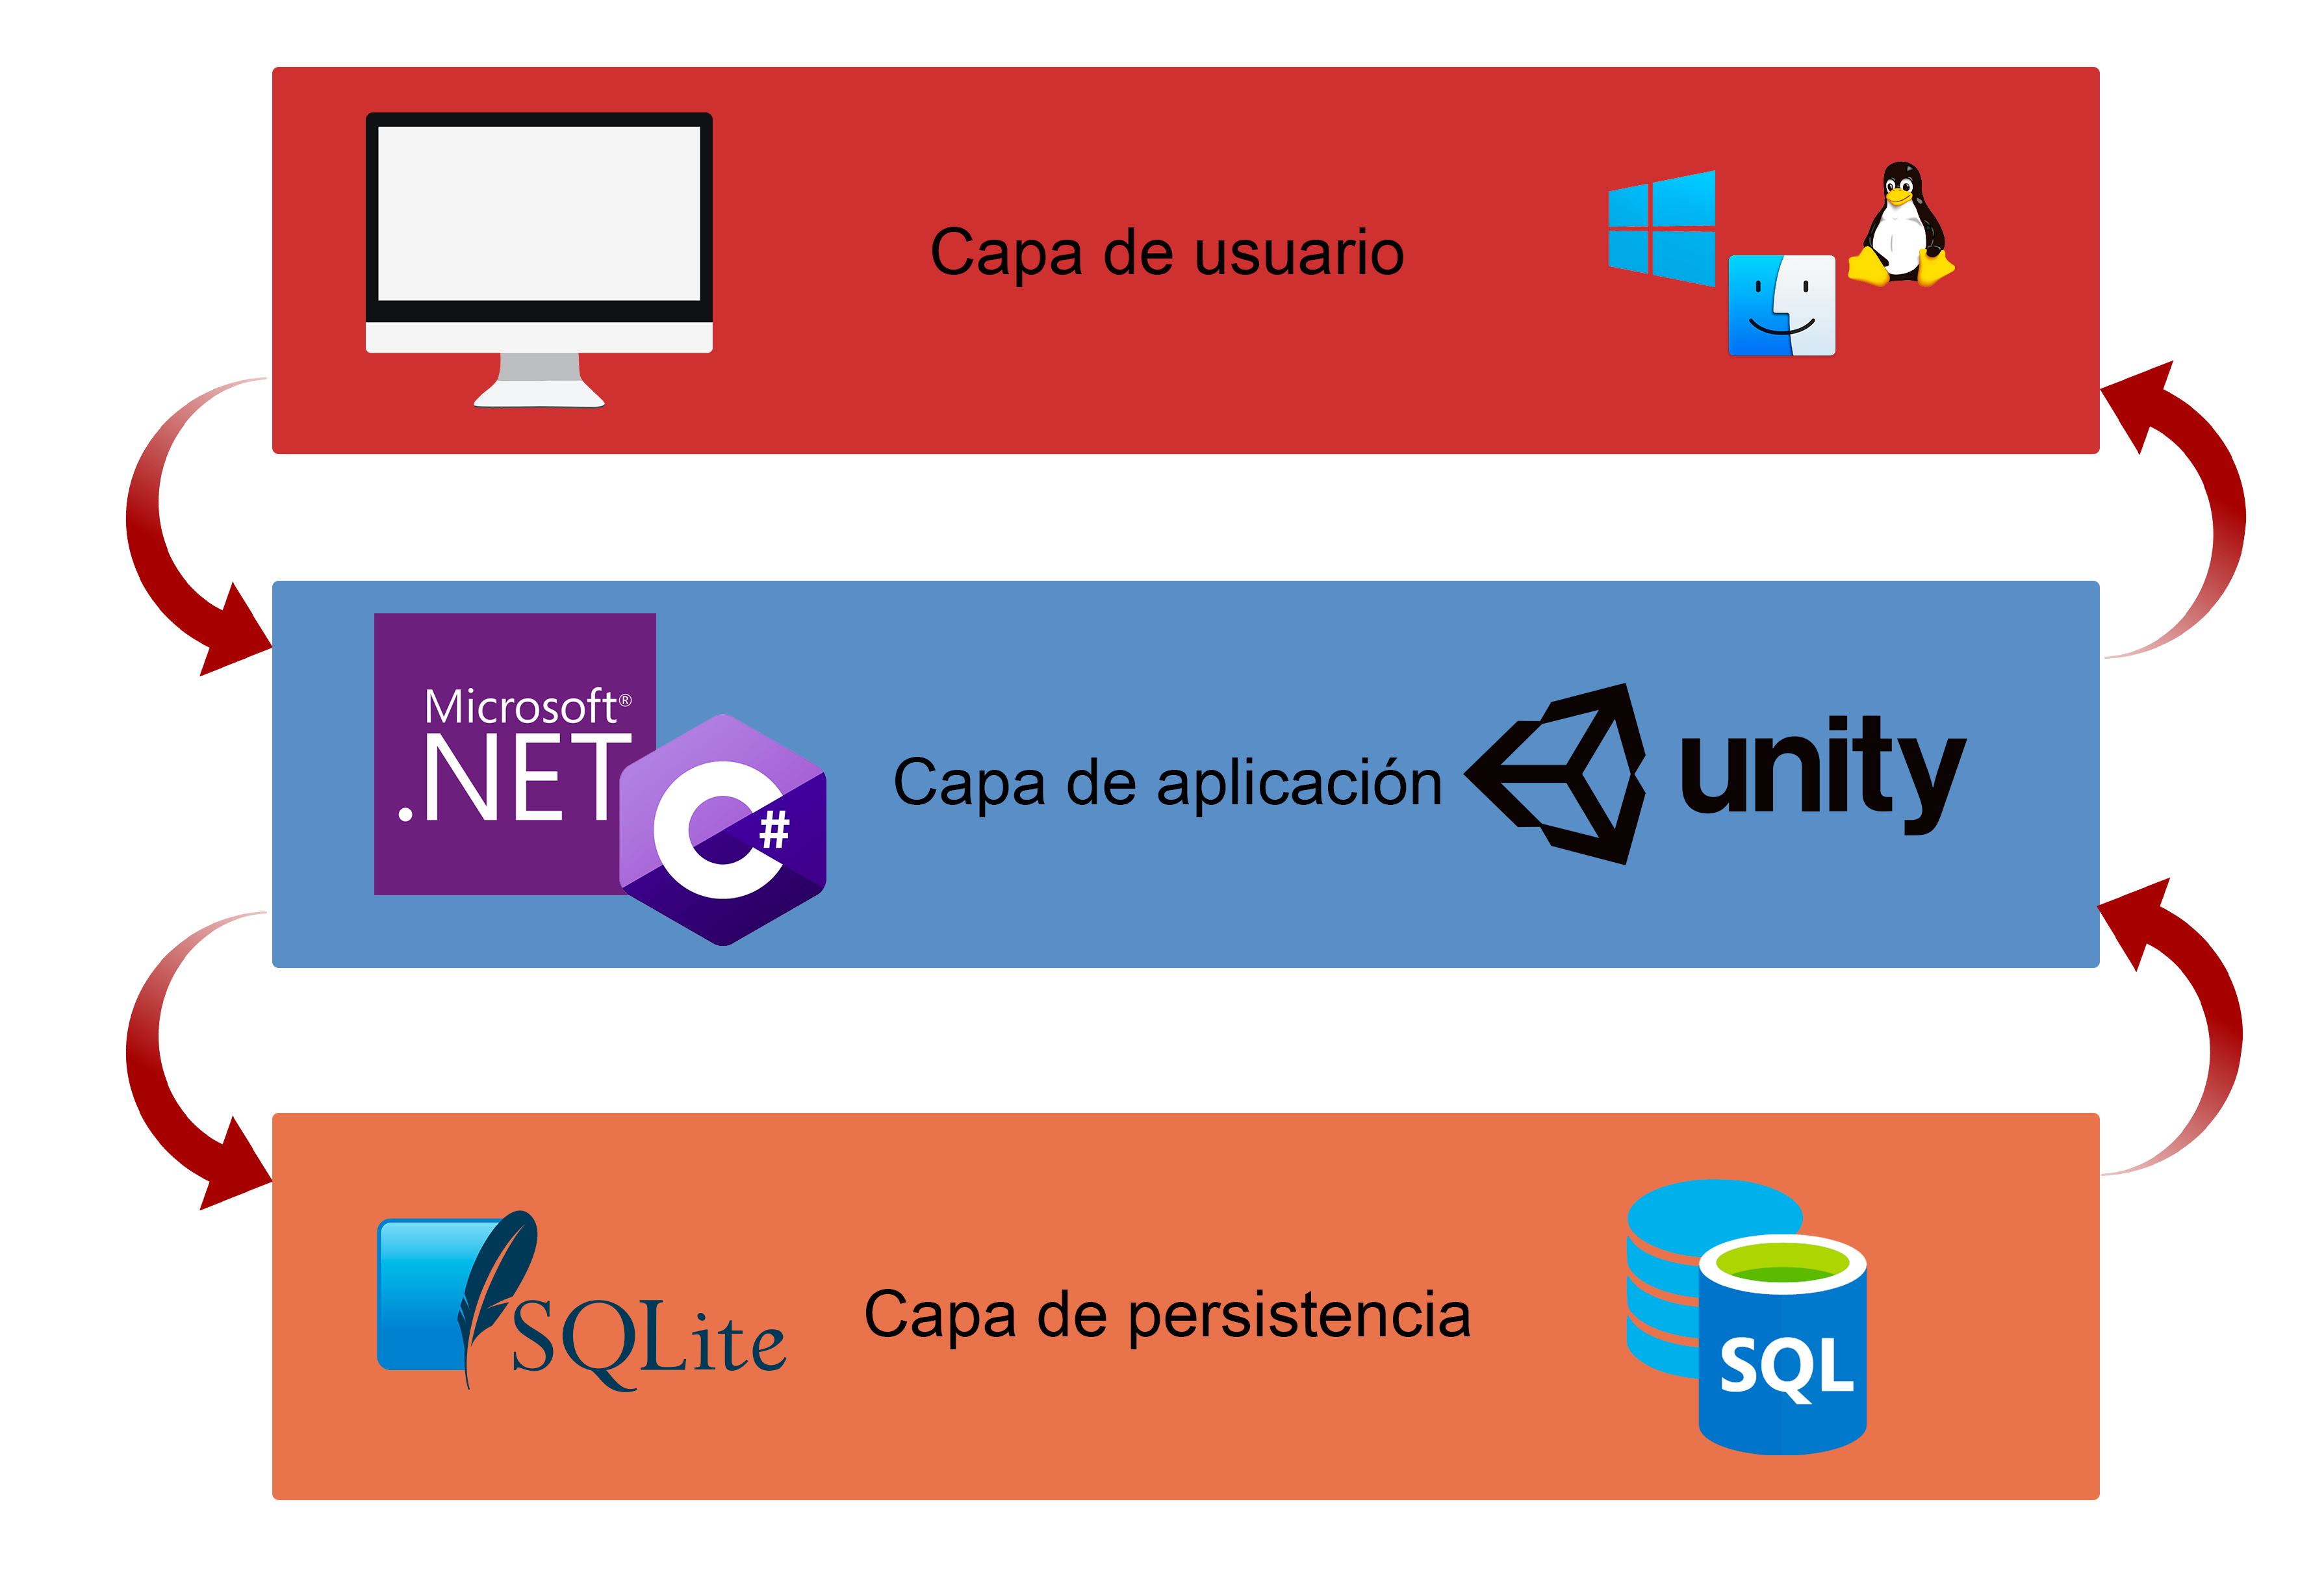
\includegraphics[width=0.95\linewidth]{ArquitecturaSoftware}
	\caption[Arquitectura software de Global-Manager]{Arquitectura software de Global-Manager}
	\label{fig:ArquitecturaSoftware}
\end{figure}

Esta arquitectura software esta compuesta por tres capas:

\begin{itemize}
	\item \textbf{Capa de usuario.} Representa el entorno sobre el cual se podrá ejecutar la aplicación. En nuestro caso, el JS consistirá en una aplicación de escritorio, la cual se podrá ejecutar en los sistemas operativos \emph{Windows}, \emph{Linux} y \emph{Mac OS}.
	\item \textbf{Capa de aplicación.} Consiste en la capa que hace referencia al JS, el cual consistirá en un proyecto \emph{.NET Framework}, en el cual se utiliza el motor de videojuegos y físicas, \emph{Unity} junto con diferentes \emph{scripts} escritos en el lenguaje de programación C\#.  
	\item \textbf{Capa de persistencia.} Esta última capa hace referencia a la base de datos o modelo de datos, donde se almacenará toda la información relevante tanto de la aplicación como de los usuarios. Para ello, se ha optado por utilizar como motor de base de datos \emph{SQLite}, de esta manera existirá una base de datos SQLite en local y se llevará a cabo el intercambio de información mediante sentencias SQL.
\end{itemize}

\subsubsection*{Componentes funcionales}
\label{sec:ComponentesFuncionales}

A continuación, se presentará una visión global del funcionamiento del juego, a través de un flujo de ejecución del juego:

\begin{enumerate}
	\item Al empezar el juego y si el jugador nunca ha jugado, este deberá rellenar un cuestionario para registrar un nuevo jugador en el sistema y obtener un nivel de usuario.
	\item Si el jugador ya tiene almacenado en el sistema un jugador, este podrá comenzar una partida seleccionando el jugador con el que desea jugar.
	\item Una partida comenzará con la ventana de configuración del proyecto, en ella, el jugador configurará un proyecto global a su gusto seleccionando y rellenando todos los componentes que aparecen en pantalla. En caso de que el jugador no sepa (debido a su bajo nivel de conocimientos) o no quiera configurar un nuevo proyecto, podrá solicitar una configuración de proyecto recomendada automáticamente en función de su nivel de jugador. Una vez, el proyecto este configurado, el jugador podrá comenzar la fase de juego.
	\item Una vez que empiece la fase de juego, se llevará a cabo una simulación de un proyecto de global y el módulo de juego proporcionará diferentes eventos que el jugador, en el rol de jefe de proyecto, deberá hacer frente y solventar.
	\item Un partida terminará exitosamente cuando se consiga la finalización del proyecto con la entrega del producto al cliente, o sin embargo, cuando el proyecto se quede sin presupuesto o no se llegue a tiempo a entregar el producto.
	\item Al finalizar la partida, el sistema proporcionara un registro con el resultado de la partida y una evaluación con el comportamiento del jugador.
	\item El jugador podrá volver a empezar otra partida.
\end{enumerate}

\section{Sprint 0}
\label{sec:Sprint0}

En primer lugar, se especificará el sprint 0 o sprint inicial, el cual servirá para detallar el alcance, planificar y sentar las bases del proyecto a desarrollar.

\subsection{Gestión de recursos humanos}
\label{sec:GestionRecursosHumanos}

En la sección \ref{sec:Roles} se definieron los roles característicos de un proyecto que utiliza Scrum como método de trabajo. Por este motivo, en este TFG se han tenido que asignar dicho roles a cada uno de los involucrados en el proyecto, asignandose los roles de "Dueño del producto", "Equipo de desarrollo" y "Scrum Master". La composición final quedaría de la siguiente manera:

\begin{table}[htbp]
\centering
\arrayrulecolor{white}
\begin{tabular}{ll}
\hline
\rowcolor[HTML]{EB6D0B} 
\multicolumn{1}{c}{\cellcolor[HTML]{EB6D0B}{\color[HTML]{FFFFFF} Rol}} & \multicolumn{1}{c}{\cellcolor[HTML]{EB6D0B}{\color[HTML]{FFFFFF} Titular/es}} \\ \hline
\rowcolor[HTML]{FFCE93} 
Dueño del producto   & Tutores del TFG \\
Equipo de desarrollo & Autor del TFG   \\
\rowcolor[HTML]{FFCE93} 
Scrum Master         & Autor del TFG   \\ \hline
\end{tabular}
\caption{Roles del equipo Scrum del proyecto}
\label{tab:RolesScrumProyecto}
\end{table}

\subsection{Planificación del proyecto}
\label{sec:PlanificacionProyecto}

Para llevar a cabo la planificación se ha procedido a crear el conjunto de historias de usuario que compondrá el proyecto. De esta manera, se pretende obtener la "Pila del Producto" (descrita en la sección \ref{sec:ComponentesScrum}). 

Una vez la pila del producto ha sido definida, es necesario establecer el conjunto de sprints del proyecto. De esta manera, se asignarán cada una de las historias de usuario a algún determinado sprint. Cada uno de los sprints estará compuesto por al menos una historia de usuario. Como resultado, se tendrá planificada la pila de cada sprint del proyecto con las historias de usuario a desarrollar. 

\subsubsection*{Pila del producto}

A continuación, se mostrará un tabla, la cual representará la pila del producto del proyecto, es decir, todas las historias de usuario que se necesitan desarrollar para obtener el producto. En la tabla \ref{tab:PilaProducto} solamente se enumeraran dichas historias de usuario junto con un valor que indicará el volumen de trabajo en días necesario para implementar dicha funcionalidad. 

\begin{table}[htbp]
\centering
\arrayrulecolor{white}
\resizebox{\textwidth}{!}{%
\begin{tabular}{rll}
\hline
\rowcolor[HTML]{EB6D0B} 
\multicolumn{1}{c}{\cellcolor[HTML]{EB6D0B}{\color[HTML]{FFFFFF} \textbf{ID}}} &
  \multicolumn{1}{c}{\cellcolor[HTML]{EB6D0B}{\color[HTML]{FFFFFF} \textbf{Título}}} &
  \multicolumn{1}{c}{\cellcolor[HTML]{EB6D0B}{\color[HTML]{FFFFFF} \textbf{Volumen}}} \\ \hline
\rowcolor[HTML]{F5D2A8} 
HDU1  & Boceto de la ventana de configuración del proyecto    & 4 días  \\
HDU2  & Boceto de la ventana de juego                         & 3 días  \\
\rowcolor[HTML]{F5D2A8} 
HDU3  & Diseñar la ventana cuestionario de nivel              & 6 días  \\
HDU4  & Diseñar la ventana de configuración del proyecto      & 8 días  \\
\rowcolor[HTML]{F5D2A8} 
HDU5  & Crear modelo 3D del teléfono, posit y lupa            & 5 días  \\
HDU6  & Diseñar la fase de juego                              & 12 días \\
\rowcolor[HTML]{F5D2A8} 
HDU7  & Diseñar la base de datos                              & 10 días \\
HDU8  & Calcular nivel del jugador                            & 5 días  \\
\rowcolor[HTML]{F5D2A8} 
HDU9  & Calcular características y dificultad del proyecto    & 6 días  \\
HDU10 & Ofrecer recomendaciones de configuración del proyecto & 8 días  \\
\rowcolor[HTML]{F5D2A8} 
HDU11 & Diseñar las preguntas de los eventos                  & 9 días  \\
HDU12 & Desarrollar flujo de juego                            & 10 días \\
\rowcolor[HTML]{F5D2A8} 
\multicolumn{1}{l}{\cellcolor[HTML]{F5D2A8}HDU13} &
  Desarrollar personalización del juego &
  15 días \\ \hline
\end{tabular}%
}
\caption{Pila del producto}
\label{tab:PilaProducto}
\end{table}

\subsubsection*{Pila de Sprints}

Justo a continuación de haber definido las historias de usuario que compondrán el desarrollo del presente proyecto, es necesario asignar cada historia de usuario a un sprint determinado, planificando así su desarrollo. En la tabla \ref{tab:PilaSprints}, se muestra el conjunto de sprints que compondrá el proyecto, junto con las historias de usuario que han de desarrollarse en cada uno y la estimación de desarrollo en días de cada sprint. Además, al final del desarrollo de cada historia de usuario se generará un artefacto resultante, el cual consistirá en un documento, boceto o prototipo de alguna funcionalidad implementada. Al final de cada sprint, todos los artefactos generados necesitan de una determinada validación para comprobar que dicha funcionalidad ha sido completada y se puede pasar a la siguiente historia de usuario.

\begin{table}[htbp]
\centering
\arrayrulecolor{white}
\resizebox{\textwidth}{!}{%
\begin{tabular}{c|c|c|l|l}
\rowcolor[HTML]{EB6D0B} 
{\color[HTML]{FFFFFF} Sprint} &
  {\color[HTML]{FFFFFF} \begin{tabular}[c]{@{}c@{}}Estimación \\ en días\end{tabular}} &
  {\color[HTML]{FFFFFF} \begin{tabular}[c]{@{}c@{}}Historias de\\ usuario\end{tabular}} &
  \multicolumn{1}{c|}{\cellcolor[HTML]{EB6D0B}{\color[HTML]{FFFFFF} \begin{tabular}[c]{@{}c@{}}Artefactos resultantes \\ del Sprint\end{tabular}}} &
  \multicolumn{1}{c}{\cellcolor[HTML]{EB6D0B}{\color[HTML]{FFFFFF} Validación}} \\ \hline
\rowcolor[HTML]{F5D2A8} 
\cellcolor[HTML]{EB6D0B}{\color[HTML]{FFFFFF} } &
  \cellcolor[HTML]{F5D2A8} &
  HDU1 &
  \begin{tabular}[c]{@{}l@{}}Boceto de la interfaz para la \\ configuración del proyecto\end{tabular} &
  Aceptación por parte del dueño del producto \\ \cline{3-5} 
\rowcolor[HTML]{F5D2A8} 
\cellcolor[HTML]{EB6D0B}{\color[HTML]{FFFFFF} } &
  \cellcolor[HTML]{F5D2A8} &
  HDU2 &
  Boceto de la interfaz de juego &
  Aceptación por parte del dueño del producto \\ \cline{3-5} 
\rowcolor[HTML]{F5D2A8} 
\multirow{-3}{*}{\cellcolor[HTML]{EB6D0B}{\color[HTML]{FFFFFF} 1}} &
  \multirow{-3}{*}{\cellcolor[HTML]{F5D2A8}17 días} &
  HDU7 &
  Base de datos &
  \begin{tabular}[c]{@{}l@{}}Alamacenados en la BBDD todos los datos \\ necesarios para llevar a cabo los cálculos del \\ juego\end{tabular} \\ \hline
\rowcolor[HTML]{F5D2A8} 
\cellcolor[HTML]{EB6D0B}{\color[HTML]{FFFFFF} } &
  \cellcolor[HTML]{F5D2A8} &
  HDU3 &
  \begin{tabular}[c]{@{}l@{}}Prototipo de la interfaz de \\ cuestionario de nivel\end{tabular} &
  Verificación por parte del dueño del producto \\ \cline{3-5} 
\rowcolor[HTML]{F5D2A8} 
\multirow{-2}{*}{\cellcolor[HTML]{EB6D0B}{\color[HTML]{FFFFFF} 2}} &
  \multirow{-2}{*}{\cellcolor[HTML]{F5D2A8}14 días} &
  HDU4 &
  \begin{tabular}[c]{@{}l@{}}Prototipo de la interfaz para la \\ configuración del proyecto\end{tabular} &
  Verificación por parte del dueño del producto \\ \hline
\rowcolor[HTML]{F5D2A8} 
\cellcolor[HTML]{EB6D0B}{\color[HTML]{FFFFFF} } &
  \cellcolor[HTML]{F5D2A8} &
  HDU8 &
  Módulo cuestionario &
  \begin{tabular}[c]{@{}l@{}}Comprobación de que se almacena en la BBDD \\ un nuevo jugador junto con un nivel acorde con \\ sus conocimientos\end{tabular} \\ \cline{3-5} 
\rowcolor[HTML]{F5D2A8} 
\cellcolor[HTML]{EB6D0B}{\color[HTML]{FFFFFF} } &
  \cellcolor[HTML]{F5D2A8} &
  HDU9 &
  \begin{tabular}[c]{@{}l@{}}Feedback entre la configuración\\ de un proyecto y su dificultad\end{tabular} &
  \begin{tabular}[c]{@{}l@{}}Comprobación de que las características y \\ dificultad de un proyecto se adaptan a su \\ configuracíon\end{tabular} \\ \cline{3-5} 
\rowcolor[HTML]{F5D2A8} 
\multirow{-3}{*}{\cellcolor[HTML]{EB6D0B}{\color[HTML]{FFFFFF} 3}} &
  \multirow{-3}{*}{\cellcolor[HTML]{F5D2A8}19 días} &
  HDU10 &
  Módulo configuración &
  \begin{tabular}[c]{@{}l@{}}Comprobación de que se ofrece una correcta \\ recomendación de configuración del proyecto \\ en función del nivel de jugador definido, \\ además de que los datos de la configuración se \\ alamcenan correctamente en la BBDD\end{tabular} \\ \hline
\rowcolor[HTML]{F5D2A8} 
\cellcolor[HTML]{EB6D0B}{\color[HTML]{FFFFFF} } &
  \cellcolor[HTML]{F5D2A8} &
  HDU5 &
  \begin{tabular}[c]{@{}l@{}}Modelo 3D de un teléfono, posit \\ y lupa, tanto en color verde como \\ en rojo\end{tabular} &
  Verificación por parte del dueño del producto \\ \cline{3-5} 
\rowcolor[HTML]{F5D2A8} 
\cellcolor[HTML]{EB6D0B}{\color[HTML]{FFFFFF} } &
  \cellcolor[HTML]{F5D2A8} &
  HDU6 &
  Prototipo de la interfaz de juego &
  Verificación por parte del dueño del producto \\ \cline{3-5} 
\rowcolor[HTML]{F5D2A8} 
\cellcolor[HTML]{EB6D0B}{\color[HTML]{FFFFFF} } &
  \cellcolor[HTML]{F5D2A8} &
  HDU11 &
  \begin{tabular}[c]{@{}l@{}}Listado de preguntas de los \\ eventos del juego\end{tabular} &
  Verificación por parte del dueño del producto \\ \cline{3-5} 
\rowcolor[HTML]{F5D2A8} 
\multirow{-4}{*}{\cellcolor[HTML]{EB6D0B}{\color[HTML]{FFFFFF} 4}} &
  \multirow{-4}{*}{\cellcolor[HTML]{F5D2A8}36 días} &
  HDU12 &
  Módulo juego &
  \begin{tabular}[c]{@{}l@{}}Comprobación de que el flujo de juego es el \\ correcto y que al final de la partida los datos \\ son almacenados en la BBDD\end{tabular} \\ \hline
\rowcolor[HTML]{F5D2A8} 
\cellcolor[HTML]{EB6D0B}{\color[HTML]{FFFFFF} 5} &
  15 días &
  HDU13 &
  Módulo inteligente &
  \begin{tabular}[c]{@{}l@{}}Comprobación de que el juego se adapta y \\ personaliza a los conocimientos del jugador\end{tabular}
\end{tabular}%
}
\caption{Pila de Sprints}
\label{tab:PilaSprints}
\end{table}

\section{Sprint 1}
\label{sec:Sprint1}

En el primer sprint del proyecto se ha considerado oportuno añadir todas las historias de usuario relacionadas con la creación de los bocetos y la idea del juego, junto con el diseño de la base de datos. De esta manera, dicho sprint sentará las bases para la creación del juego Global-Manager. Cabe destacar que durante el desarrollo del presente sprint se han realizado los cambios pertinentes ofrecidos por el dueño del producto tras mostrarle los diseños de los bocetos y la base de datos.

\subsection{Planificación del Sprint}
\label{sec:PlanifiacionSprint1}

A continuación, se muestra la planificación que se ha seguido para el desarrollo del presente sprint. Para llevar a cabo dicha planificación, se ha obtenido la pila del sprint 1, anteriormente descrita en la sección \ref{sec:PlanificacionProyecto}, y se han completado las historias de usuario con un mayor nivel de detalle. Las historias de usuario que se desarrollaran en el sprint 1 son las siguientes:

\begin{table}[htbp]
\centering
\arrayrulecolor{white}
\resizebox{\textwidth}{!}{%
\begin{tabular}{ccc}
\rowcolor[HTML]{EB6D0B} 
\multicolumn{1}{c|}{\cellcolor[HTML]{EB6D0B}{\color[HTML]{FFFFFF} Sprint 1}} &
  \multicolumn{1}{c|}{\cellcolor[HTML]{EB6D0B}{\color[HTML]{FFFFFF} HDU1}} &
  \cellcolor[HTML]{F5D2A8}{\color[HTML]{333333} Boceto de la ventana de configuración del proyecto} \\ \hline
\rowcolor[HTML]{EB6D0B} 
\multicolumn{3}{c}{\cellcolor[HTML]{EB6D0B}{\color[HTML]{FFFFFF} Descripción}} \\ \hline
\rowcolor[HTML]{F5D2A8} 
\multicolumn{3}{l}{\cellcolor[HTML]{F5D2A8}\begin{tabular}[c]{@{}l@{}}Quiero ver un diseño gráfico mediante un boceto de una ventana que me permita visualizar todos los componentes \\ para la configuración de un proyecto de DGS para dar feedback antes de comenzar la implementación\end{tabular}} \\ \hline
\rowcolor[HTML]{EB6D0B} 
\multicolumn{3}{c}{\cellcolor[HTML]{EB6D0B}{\color[HTML]{FFFFFF} Resumen de las tareas}} \\ \hline
\rowcolor[HTML]{F5D2A8} 
\multicolumn{3}{l}{\cellcolor[HTML]{F5D2A8}\begin{tabular}[c]{@{}l@{}}- Diseñar parte del boceto para la configuación inicial del proyecto\\  - Diseñar parte del boceto para la configuración de cada site\\  - Diseñar parte del boceto para la configuración de la comunicación entre sites\\  - Diseñar parte del boceto para la visualización de las caracteristicas del proyecto\\  - Diseñar parte del boceto para la visualización de la dificultad del proyecto\\  - Presentar resultados al dueño del producto\\  - Modificar los cambios propuestos\end{tabular}} \\ \hline
\rowcolor[HTML]{EB6D0B} 
\multicolumn{1}{c|}{\cellcolor[HTML]{EB6D0B}{\color[HTML]{FFFFFF} Estimación}} &
  \multicolumn{1}{c|}{\cellcolor[HTML]{EB6D0B}{\color[HTML]{FFFFFF} Valor (1/10)}} &
  {\color[HTML]{FFFFFF} Dependencias} \\ \hline
\rowcolor[HTML]{F5D2A8} 
\multicolumn{1}{c|}{\cellcolor[HTML]{F5D2A8}4 días} &
  \multicolumn{1}{c|}{\cellcolor[HTML]{F5D2A8}5} &
  -
\end{tabular}%
}
\caption{Historia de usuario 1: Boceto de la ventana de configuración del proyecto}
\label{tab:HDU1}
\end{table}

\begin{table}[htbp]
\centering
\arrayrulecolor{white}
\resizebox{\textwidth}{!}{%
\begin{tabular}{ccc}
\rowcolor[HTML]{EB6D0B} 
\multicolumn{1}{c|}{\cellcolor[HTML]{EB6D0B}{\color[HTML]{FFFFFF} Sprint 1}} &
  \multicolumn{1}{c|}{\cellcolor[HTML]{EB6D0B}{\color[HTML]{FFFFFF} HDU2}} &
  \cellcolor[HTML]{F5D2A8}{\color[HTML]{333333} Boceto de la ventana de juego} \\ \hline
\rowcolor[HTML]{EB6D0B} 
\multicolumn{3}{c}{\cellcolor[HTML]{EB6D0B}{\color[HTML]{FFFFFF} Descripción}}                           \\ \hline
\rowcolor[HTML]{F5D2A8} 
\multicolumn{3}{l}{\cellcolor[HTML]{F5D2A8}\begin{tabular}[c]{@{}l@{}}Quiero ver un diseño gráfico mediante un boceto de la ventana de juego donde aparezca el avatar de un jugador y\\ distintos objetos (que representen situaciones de un proyecto de DGS) puedan caer sobre el escenario de juego\end{tabular}} \\ \hline
\rowcolor[HTML]{EB6D0B} 
\multicolumn{3}{c}{\cellcolor[HTML]{EB6D0B}{\color[HTML]{FFFFFF} Resumen de las tareas}}                 \\ \hline
\rowcolor[HTML]{F5D2A8} 
\multicolumn{3}{l}{\cellcolor[HTML]{F5D2A8}\begin{tabular}[c]{@{}l@{}}- Diseñar boceto del avatar de juego\\  - Diseñar boceto del escenario de juego\\  - Diseñar los objetos\\  - Presentar resultados al dueño del producto\\  - Modificar los cambios propuestos\end{tabular}} \\ \hline
\rowcolor[HTML]{EB6D0B} 
\multicolumn{1}{c|}{\cellcolor[HTML]{EB6D0B}{\color[HTML]{FFFFFF} Estimación}} &
  \multicolumn{1}{c|}{\cellcolor[HTML]{EB6D0B}{\color[HTML]{FFFFFF} Valor (1/10)}} &
  {\color[HTML]{FFFFFF} Dependencias} \\ \hline
\rowcolor[HTML]{F5D2A8} 
\multicolumn{1}{c|}{\cellcolor[HTML]{F5D2A8}3 días} & \multicolumn{1}{c|}{\cellcolor[HTML]{F5D2A8}6} & -
\end{tabular}%
}
\caption{Historia de usuario 2: Boceto de la ventana de juego}
\label{tab:HDU2}
\end{table}

\begin{table}[htbp]
\centering
\resizebox{\textwidth}{!}{%
\begin{tabular}{ccc}
\rowcolor[HTML]{EB6D0B} 
\multicolumn{1}{c|}{\cellcolor[HTML]{EB6D0B}{\color[HTML]{FFFFFF} Sprint 1}} &
  \multicolumn{1}{c|}{\cellcolor[HTML]{EB6D0B}{\color[HTML]{FFFFFF} HDU7}} &
  \cellcolor[HTML]{F5D2A8}{\color[HTML]{333333} Diseñar la base de datos} \\ \hline
\rowcolor[HTML]{EB6D0B} 
\multicolumn{3}{c}{\cellcolor[HTML]{EB6D0B}{\color[HTML]{FFFFFF} Descripción}} \\ \hline
\rowcolor[HTML]{F5D2A8} 
\multicolumn{3}{l}{\cellcolor[HTML]{F5D2A8}\begin{tabular}[c]{@{}l@{}}Quiero una base de datos donde pueda almacenar la información de cada jugador, las configuraciones de los \\ proyectos y las partidas que se desarrollan en el juego. Además, se tienen que almacenar los datos necesarios\\ para realizar los diferentes cálculos que se llevan a cabo a lo largo del juego\end{tabular}} \\ \hline
\rowcolor[HTML]{EB6D0B} 
\multicolumn{3}{c}{\cellcolor[HTML]{EB6D0B}{\color[HTML]{FFFFFF} Resumen de las tareas}} \\ \hline
\rowcolor[HTML]{F5D2A8} 
\multicolumn{3}{l}{\cellcolor[HTML]{F5D2A8}\begin{tabular}[c]{@{}l@{}}- Diseñar el almacenamiento de los jugadores\\  - Diseñar el almacenamiento de las configuraciones de los proyectos\\  - Diseñar el almacenamiento de las partidas jugadas\\  - Introducir los datos necesarios para el juego\\  - Presentar resultados al dueño del producto\\  - Modificar los cambios propuestos\end{tabular}} \\ \hline
\rowcolor[HTML]{EB6D0B} 
\multicolumn{1}{c|}{\cellcolor[HTML]{EB6D0B}{\color[HTML]{FFFFFF} Estimación}} &
  \multicolumn{1}{c|}{\cellcolor[HTML]{EB6D0B}{\color[HTML]{FFFFFF} Valor (1/10)}} &
  {\color[HTML]{FFFFFF} Dependencias} \\ \hline
\rowcolor[HTML]{F5D2A8} 
\multicolumn{1}{c|}{\cellcolor[HTML]{F5D2A8}10 días} &
  \multicolumn{1}{c|}{\cellcolor[HTML]{F5D2A8}10} &
  -
\end{tabular}%
}
\caption{Historia de usuario 3: Diseñar la base de datos}
\label{tab:HDU3}
\end{table}

Tras la finalización del presente sprint se obtendrán como resultado los siguientes artefactos:
\begin{itemize}
	\item Boceto de la interfaz para la configuración del proyecto
	\item Boceto de la interfaz de juego
	\item Base de datos
\end{itemize}

\subsection{HDU1 - Boceto de la ventana de configuración del proyecto}
\label{sec:HDU1}

En esta primera historia de usuario a desarrollar se lleva a cabo el diseño del boceto de una de las interfaces principales de Global-Manager, la cual será la ventana de configuración de un proyecto, cuya utilidad servirá para ofrecer al jugador la oportunidad de crear sus propias partidas personalizadas por él. Dicho boceto pretenderá dar una idea general del concepto del juego, comprender como se introducirán los conocimientos que queremos enseñar y ayudar a entender los diseños técnicos.

Para crear los conceptos e idea de Global-Manager, se han evaluado diferentes JS existentes en el estado del arte, parecidos a la temática de nuestro juego, en donde se enseñan conceptos de DGS o se aprenden a gestionar proyectos software. De esta manera, se pretende ampliar las funcionalidades que ya ofrecen los JS existentes (véase la sección \ref{sec:TrabajosRelacionados}).

Para la elaboración del diseño de los bocetos de las interfaces de Global-Manager, se ha utilizado la herramienta de diseño de interfaces \emph{Balsamiq Mockups}.

\label{sec:HDU2}

\subsection{HDU7 - Diseñar la base de datos}
\label{sec:HDU7}